\documentclass{article}
\usepackage[english]{babel} % Changed to English
\usepackage[T1]{fontenc}
\usepackage{graphicx}   % For including images
\usepackage{fancyhdr}   % For customizing headers and footers
\usepackage{tabularx}
\usepackage{subcaption} % For subcaptions in figures
\usepackage{placeins}   % For \FloatBarrier to control float placement
\usepackage{float}
\usepackage{wrapfig}    % For wrapfigure environment
\usepackage{tikz}       % For drawing diagrams
\usetikzlibrary{decorations.pathreplacing} % For brace decoration in TikZ
\usetikzlibrary{angles, quotes, positioning, arrows.meta}   
\usetikzlibrary{calc} % For coordinate calculations in TikZ
\usepackage{amsmath}    % For \text and other math features
\usepackage{booktabs}   % For \toprule, \midrule, \bottomrule in tables
% \usepackage{bibentry}
% \nobibliography*
\usepackage{url}
\usepackage[hidelinks]{hyperref}
\hypersetup{urlcolor=blue}
\usepackage[numbers]{natbib}
\usepackage{doi}
\usepackage{titlesec} % Added for \titleformat command

% Suppress subfigure labels (a), (b), etc.
\captionsetup[subfigure]{labelformat=empty}

% Set up the header and footer
\fancyfoot[R]{
\includegraphics[height=.75cm]{imgs/unilr_logo.png}} % Logo on the right
\fancyfoot[L]{NGUYEN Hoang Nhat}                             % Name on the left
\fancyfoot[C]{\thepage}                              % Page number centered
\renewcommand{\footrulewidth}{0.5pt}                 % Line above footer
\renewcommand{\headrulewidth}{0pt}                   % Remove the header line
\fancyhead{}                                         % Clear all header content
\pagestyle{fancy}                                    % Apply fancy style to all pages after title

% Beginning the document
\begin{document}
\pagenumbering{gobble} % Suppress page numbering on the title page

% Centering all content for the cover page
\begin{center}

% Including logos side by side
\begin{minipage}{0.7\textwidth}
    
\includegraphics[height=3cm]{imgs/mia_logo.png}
    \hfill
\end{minipage}
\hfill
\begin{minipage}{0.29\textwidth}
    \hfill
    
\includegraphics[height=3cm]{imgs/unilr_logo.png}
\end{minipage}
\vspace{1cm}

% Adding horizontal lines above and below the title section
\noindent\rule{\textwidth}{2pt}

% Adding the title of the report
{\Huge \textbf{Internship Report (Extra)}\par}
\vspace{1cm}

% Adding the specific topic of the internship
{\Large \textbf{Detection and Semantic Segmentation on Meta Quest 3}\par}

\noindent\rule{\textwidth}{2pt}

\vspace{1cm}

% Adding the author's name
{\Huge \textbf{NGUYEN Hoang Nhat}\par}
\vspace{1cm}

% Adding the internship period
{\large \textbf{Internship Period: April 20, 2026 -- June 19, 2026}\par}
\vspace{1cm}

% Adding the institution and laboratory details
{\large \textbf{Laboratoire Mathématiques, Image et Applications}\par}
{\large \textbf{La Rochelle Université}\par}
\vspace{1.5cm}

\begin{minipage}{0.49\textwidth}
    \raggedright
    {\large \textbf{Submitted on:}\\ 29/5/2026\par}
\end{minipage}
\begin{minipage}{0.49\textwidth}
    \raggedleft
    {\large \textbf{Supervisor:}\\ Péteri Renaud }\\
    {\large \textbf{University tutor:}\\ Mascarilla Laurent  }
\end{minipage}

\end{center}

% Ensuring no page number appears
\thispagestyle{empty}


\newpage
\tableofcontents

\newpage

\section{Code Explanation}

\subsection{Execution Flow}

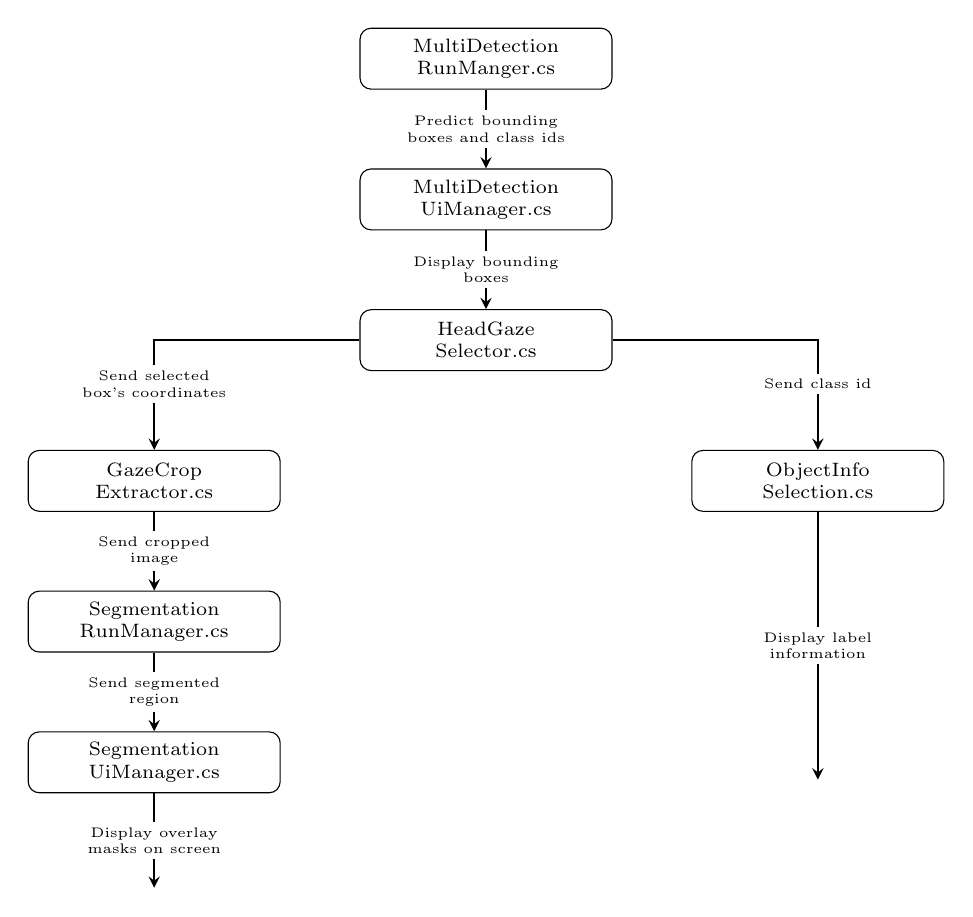
\begin{tikzpicture}[
    % Reduced horizontal gap from 1.2cm to 0.3cm
    node distance=1cm and 1cm, 
    % Reduced box width from 4.2cm to 3.2cm
    box/.style={rectangle, draw, rounded corners, align=center, minimum width=3.2cm, minimum height=2.2em, font=\scriptsize},
    arrow/.style={-stealth, thick},
    lbl/.style={font=\tiny, fill=white, inner sep=2pt, align=center}
]
    % --- Core Nodes Layout (Text wrapped to stay inside smaller boxes) ---
    \node[box] (b1) {MultiDetection\\RunManger.cs};
    \node[box] (b2) [below=of b1] {MultiDetection\\UiManager.cs};
    \node[box] (b3) [below=of b2] {HeadGaze\\Selector.cs};
    
    % Branching layout below HeadGazeSelector
    \node[box] (b4) [below left=of b3] {GazeCrop\\Extractor.cs};
    \node[box] (b4_1) [below right=of b3] {ObjectInfo\\Selection.cs};
    
    % Sub-branch files neatly positioned downward
    \node[box] (b5) [below=of b4] {Segmentation\\RunManager.cs};
    \node[box] (b6) [below=of b5] {Segmentation\\UiManager.cs};

    % --- Invisible Destination Points for Output Arrows ---
    \coordinate [below=1.2cm of b6] (out_left);
    \coordinate [below=3.4cm of b4_1] (out_right);

    % --- Arrow Connections with Text Labels (Wrapped to prevent wide spacing) ---
    \draw[arrow] (b1) -- node[lbl] {Predict bounding\\boxes and class ids} (b2);
    \draw[arrow] (b2) -- node[lbl] {Display bounding\\boxes} (b3);
    
    % --- Left and Right Branch Labels ---
    \draw[arrow] (b3) -| node[lbl, pos=0.7] {Send selected\\box's coordinates} (b4);
    \draw[arrow] (b3) -| node[lbl, pos=0.7] {Send class id} (b4_1);
    
    % --- Bottom Pipeline Connections ---
    \draw[arrow] (b4) -- node[lbl] {Send cropped\\image} (b5);
    \draw[arrow] (b5) -- node[lbl] {Send segmented\\region} (b6);
    
    % --- Ending Nodes Output Arrows ---
    \draw[arrow] (b6) -- node[lbl] {Display overlay\\masks on screen} (out_left);
    \draw[arrow] (b4_1) -- node[lbl] {Display label\\information} (out_right);
    
\end{tikzpicture}

The pipeline is split into two parallel stages. The detection stage runs continuously on every other camera frame, while the segmentation stage is triggered on demand only when the user selects a bounding box with their head gaze. The following subsections describe each script in pipeline order.

%──────────────────────────────────────────────────────────────────
\subsection{Detection Stage}
%──────────────────────────────────────────────────────────────────

\subsubsection{\texttt{MultiDetectionRunManager.cs} - Inference Loop}

This script is the entry point of the real-time detection pipeline. Every frame it retrieves the live passthrough camera texture from the \texttt{PassthroughCameraAccess}, copies it into a pre-allocated \texttt{Tensor<float>} of shape $(1,3,1280,1280)$, and schedules it through a Unity Sentis \texttt{Worker} backed by the Vulkan compute backend (\texttt{GPUCompute}).

The ONNX model (YOLOv8n) is converted to the \texttt{.sentis} format in the Editor by \texttt{DetectionModelEditorConverter.cs}, which appends a centers-to-corners matrix multiplication layer so that bounding-box coordinates arrive in $(x_1, y_1, x_2, y_2)$ corner format rather than the native $(c_x, c_y, w, h)$ format. This avoids the conversion cost at runtime on every frame.

The model produces three output tensors - corners, class IDs, and confidence scores - whose GPU-to-CPU readbacks are issued simultaneously and awaited in parallel inside a coroutine, minimising GPU pipeline stalls. Once the data arrives on the CPU, a standard greedy Non-Maximum Suppression (NMS) pass is applied using pre-allocated working lists (no per-frame heap allocations), and the surviving detections are forwarded to \texttt{MultiDetectionUiManager}.

\subsubsection{\texttt{MultiDetectionUiManager.cs} - Bounding Box Rendering}

This script translates the 2D pixel-space detections into world-space bounding boxes anchored to real surfaces. For each detection, the normalised viewport center is converted to a 3D ray via \texttt{PassthroughCameraAccess.ViewportPointToRay}, which internally uses the camera's calibrated intrinsics. The ray is then intersected with the environment mesh by \texttt{EnvironmentRayCastSampleManager} to obtain a world-space hit point.

To determine the physical size of the box, the four corner rays of the detection rectangle are intersected with a plane perpendicular to the camera direction at the depth of the hit point. The resulting world-space corner offsets are projected into the camera's local coordinate frame to extract a 2D width and height. A \texttt{RectTransform} prefab is then placed at the hit point, oriented to face the camera, and sized to these world-space dimensions.

A pooling system avoids instantiating new \texttt{GameObject}s on every frame: existing boxes are reused when a new detection overlaps them (IoU~$> 0$) and belongs to the same class, or removed when a different class occupies the same region (IoU~$> 0.1$). Boxes that have not been updated for 750\,ms are automatically returned to the pool.

Each \texttt{BoundingBoxData} record also stores the detection's normalised bounding-box coordinates (the \texttt{NormalizedBBox} field), which are passed downstream to the crop extractor.

%──────────────────────────────────────────────────────────────────
\subsection{Gaze Selection}
%──────────────────────────────────────────────────────────────────

\subsubsection{\texttt{HeadGazeSelector.cs} - Gaze Ray Casting}

This script implements a hands-free selection mechanism. Each frame it constructs a ray from the \texttt{CenterEyeAnchor} transform (representing the user's head direction) and tests it against every active bounding box managed by \texttt{MultiDetectionUiManager}.

For each box, the perpendicular distance from the gaze ray to the box's world-space center is compared against a hit radius defined as half the diagonal of the box's world-space size. Among all boxes that pass this test, the one whose center subtends the smallest angle with the gaze direction is selected. A color change on the box's \texttt{Image} component provides visual feedback, and an \texttt{OnSelectionChanged} event is fired whenever the selection changes. The two downstream consumers - \texttt{GazeCropExtractor} and \texttt{ObjectInfoSelection} - both subscribe to this event.

%──────────────────────────────────────────────────────────────────
\subsection{Right Branch - Object Information Display}
%──────────────────────────────────────────────────────────────────

\subsubsection{\texttt{ObjectInfoDatabase.cs} and \texttt{ObjectInfoEntry.cs} - JSON Metadata}

\texttt{ObjectInfoDatabase} parses a JSON asset at startup. The root object is expected to contain a \texttt{"classes"} array; any other top-level keys (e.g.\ \texttt{"metadata"}) are ignored. Each element is deserialised into an \texttt{ObjectInfoEntry} instance using Newtonsoft.Json and stored in a dictionary keyed by integer class ID.

\texttt{ObjectInfoEntry} is the data model. It captures per-class metadata used for display: canonical name, aliases, material composition, 3D shape profile (geometry and symmetry), typical physical dimensions in centimetres, segmentation difficulty and recommended approach, occlusion risk, and pose estimation notes.

\subsubsection{\texttt{ObjectInfoSelection.cs} - Info Panel}

When \texttt{HeadGazeSelector} fires \texttt{OnSelectionChanged}, this script looks up the selected class ID in \texttt{ObjectInfoDatabase} and formats a rich-text string (using Unity's legacy \texttt{Text} component with bold and italic tags). The info panel - a world-space \texttt{Canvas} child - is then activated, sized to fixed world-space dimensions, and positioned flush to the right edge of the selected bounding box with a configurable gap. Each frame the panel follows the box using a \texttt{Vector3.Lerp} and billboards to face the main camera.

%──────────────────────────────────────────────────────────────────
\subsection{Left Branch - Segmentation Pipeline}
%──────────────────────────────────────────────────────────────────

\subsubsection{\texttt{GazeCropExtractor.cs} - ROI Cropping and Letterboxing}

This script runs at a configurable interval (default 100\,ms) rather than every frame to avoid saturating the GPU with segmentation inference requests. When the gaze selection is non-null, it crops the padded bounding-box region from the live camera texture using two sequential GPU \texttt{Graphics.Blit} calls.

The first blit extracts the raw crop at native pixel resolution. The second applies a letterbox resize: a uniform scale factor $s = \min(1,\, T/w,\, T/h)$ is computed where $T = 640$ is the model input size and $w, h$ are the crop dimensions. This ensures larger crops are scaled down to fit while smaller crops are padded without upscaling. The output is always a $640 \times 640$ \texttt{RenderTexture} with black padding bars on the shorter axis.

Both the viewport coordinates of the original padded bbox in camera space and the UV sub-rect of the real-image content inside the $640 \times 640$ texture are stored in a \texttt{CropInfo} struct and forwarded to \texttt{SegmentationRunManager} via the \texttt{OnCropReady} event. The UV sub-rect is essential for the overlay placement step, allowing the downstream UI manager to display only the content region of the mask texture.

\subsubsection{\texttt{SegmentationRunManager.cs} - Segmentation Inference}

This script supports two operating modes selectable via a single Inspector toggle.

\paragraph{Semantic mode (YOLO26n-sem).}
The model outputs a single tensor of shape $(1, C, H, W)$ containing per-pixel class logits. An argmax over the class dimension $C$ produces a flat integer array \texttt{classMap} of size $H \times W$. A validity check ensures the target class ID (the one gaze-selected by the user) is present in the map before the result is fired; frames where the object is absent are silently dropped.

\paragraph{(Optional) Instance mode (YOLO26n-seg).}
The model outputs two tensors: detections of shape $(1, 4 + C + 32, 8400)$ and prototype masks of shape $(1, 32, H_p, W_p)$. Only anchors whose score for the target class exceeds a configurable threshold are kept. These are sorted by score and deduplicated with NMS. For the surviving best detection, its 32 mask coefficients are combined with the prototype masks via a dot product followed by a sigmoid, producing a continuous mask at prototype resolution. Pixels above a configurable threshold (default 0.5) are labelled with the target class ID; all others are set to background. The mask is then cropped to the detection bounding box projected onto prototype space to suppress leakage outside the object extent.

Both modes produce a \texttt{SegResult} struct with the same fields - \texttt{classMap}, map dimensions, target class ID, class label, the crop viewport rect, and the letterbox UV rect - so the downstream UI manager is mode-agnostic.

A debug placeholder mode bypasses inference entirely and fires a placeholder \texttt{SegResult} (with a null \texttt{classMap}), allowing the UI placement logic to be verified independently of a working model.

\subsubsection{\texttt{SegmentationUiManager.cs} - Mask Overlay Rendering}

Upon receiving a \texttt{SegResult}, this script offloads pixel colouring to a background thread-pool task (\texttt{Task.Run}) to avoid blocking the Unity main thread. The task iterates over the \texttt{classMap} and writes a semi-transparent color into a \texttt{Color32} array: pixels whose class ID matches the target receive an HSV-derived tint unique to that class ID; all others are written as fully transparent. A vertical flip is applied during iteration because model output row 0 is the top of the image while \texttt{Texture2D} row 0 is the bottom.

When the task completes the main thread uploads the pixel array to a reused \texttt{Texture2D} and calls \texttt{PlaceOverlay}. This method replicates the same world-space projection logic used for bounding boxes: the crop viewport corners are cast as rays, intersected with a plane at the environment-raycast depth, and the resulting world-space size is assigned to the overlay \texttt{RectTransform}'s \texttt{sizeDelta}. Crucially, \texttt{RawImage.uvRect} is set to \texttt{ModelInputUVRect} so that only the letterbox-content region of the $640 \times 640$ texture is displayed, making the mask pixel-accurately aligned with the underlying bounding box.

A serial number is incremented each time a new result arrives; stale completions (from a previous result whose task finished after a newer one began) are discarded before the texture upload, preventing flickering from out-of-order deliveries.

\section{Fixes}
This section describes the work done after the internship defense and towards the end of my internship.

\subsection{Finishing Model finetuning}
The dataset's images were changed to match the size of the frame input: 1280x1280 for detection and 640x640 for segmentation. The script for resizing can be found in \href{https://github.com/NguyenHoangNhat-git/Segmentation-and-Multi-Detection-YOLO-for-Meta-Quest-3}{\textbf{My Github}}

\subsubsection{Detection}
Every hyperparameter and data augmentation configuration were kept the same, except for the `imgsize` which is now set to 640x640.

\paragraph{Results.}
The fine-tuned model was evaluated during training on the validation set at IoU threshold 0.5 and 0.5-0.95, which is shown in Figure~\ref{fig:det-finetune-mAP}. 
The resulting model was then evaluated on the held-out test set, and per-class metrics are reported in Table~\ref{tab:det-finetune-results}.

\begin{figure}[H]
    \centering
    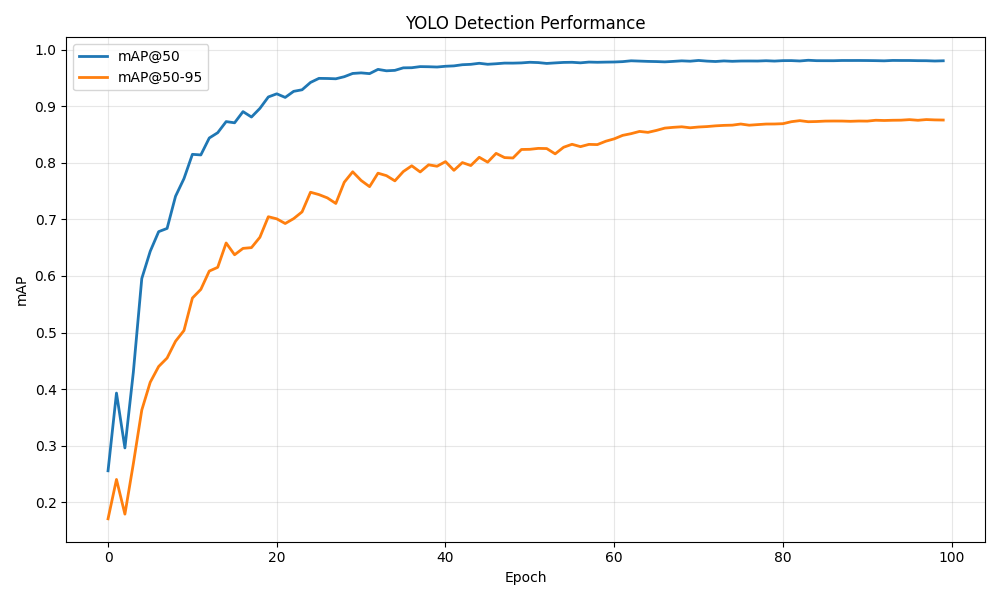
\includegraphics[width=\linewidth]{imgs/det_map.png}
    \caption{Mean AVerage Precision at threshold 0.5 and 0.5-0.95 on the validation set during training over 100 epochs}
    \label{fig:finetune-curves}

    \vspace{1cm}
    
    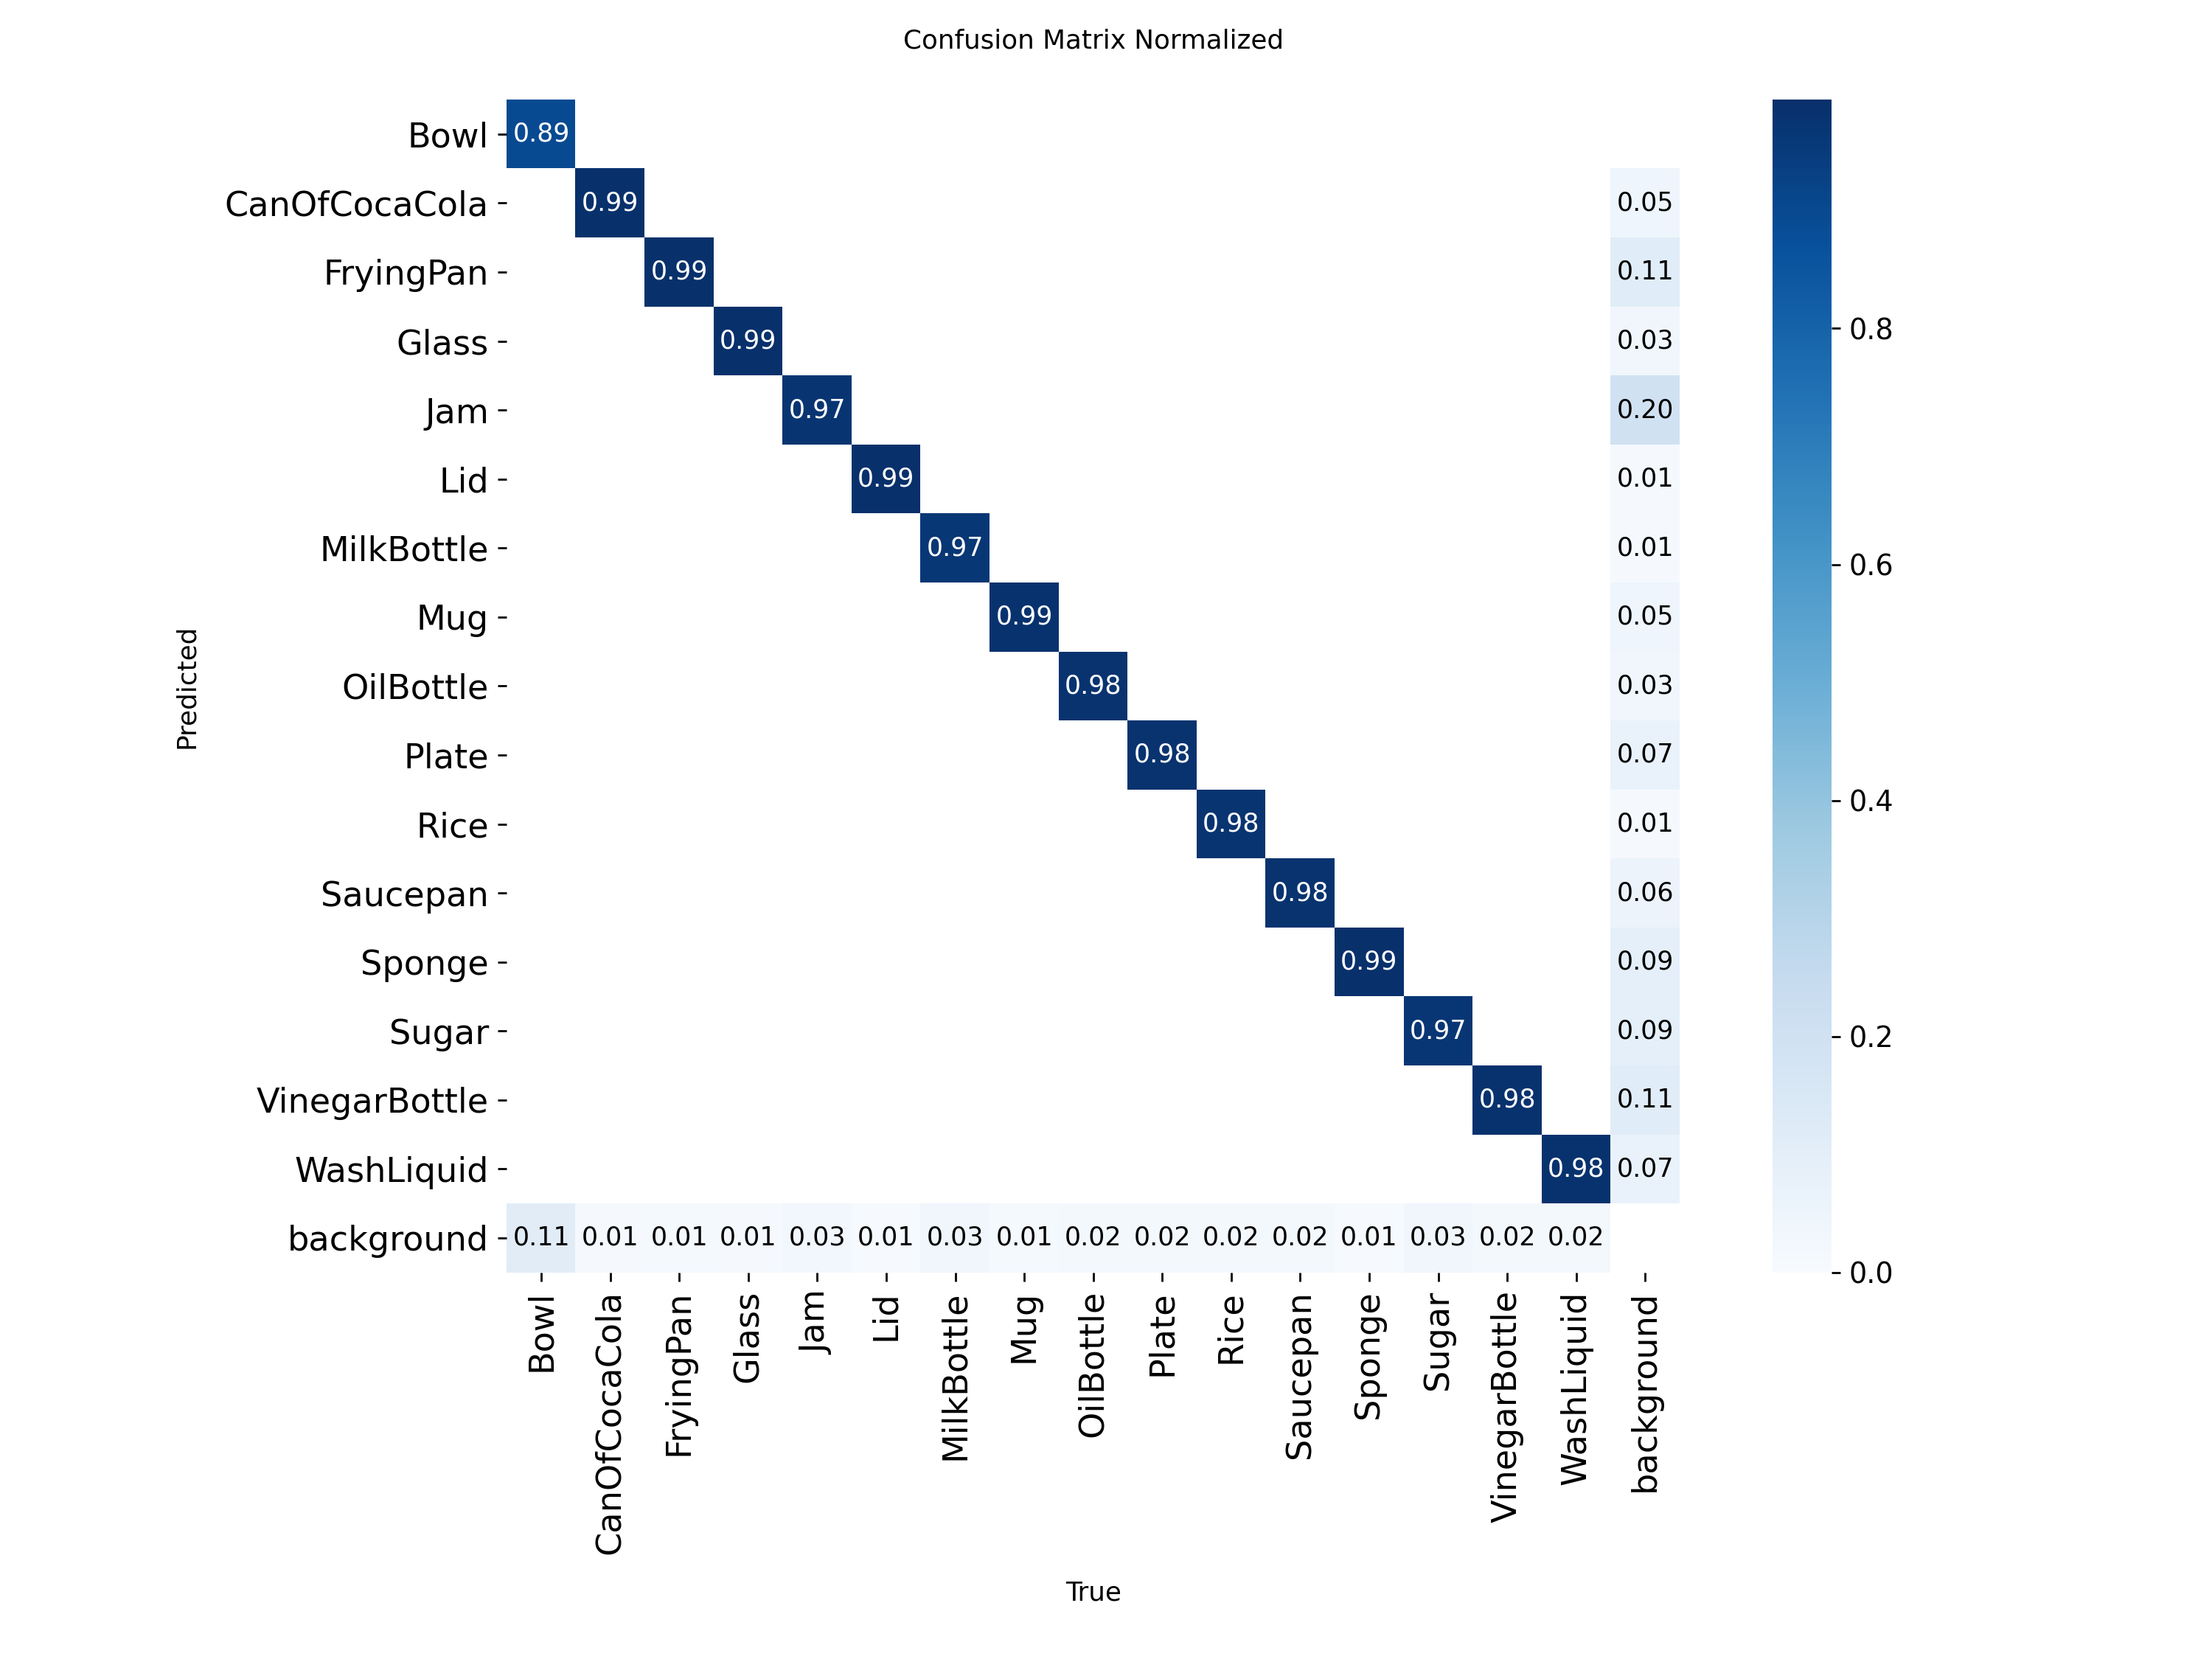
\includegraphics[width=\linewidth]{imgs/det_conf_norm_mat.png}
    \caption{Normalized Confusion matrix on the validation set}
    \label{fig:finetune-confmat}
\end{figure}

\subsubsection{Semantic Segmentation}
Every hyperparameter and data augmentation configuration were kept the same, except for the `imgsize` which is now set to 1280x1280. Note that this matches the resolution of the newest \textbf{HorizonOS v83}.

\paragraph{Results.}
The fine-tuned model was evaluated on the held-out test set. Training and validation curves are shown in Figure~\ref{fig:finetune-curves}. The results are excellent, reaching a mIoU of \textbf{0.98}. 

\begin{figure}[H]
    \centering
    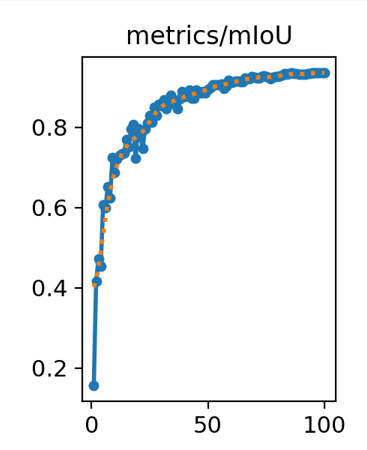
\includegraphics[width=0.4\linewidth]{imgs/sem_finetuning_IoU.png}
    \caption{Mean Intersection over Union (mIoU) on the validation set during training over 100 epochs}
    \label{fig:finetune-curves}

    \vspace{1cm}
    
    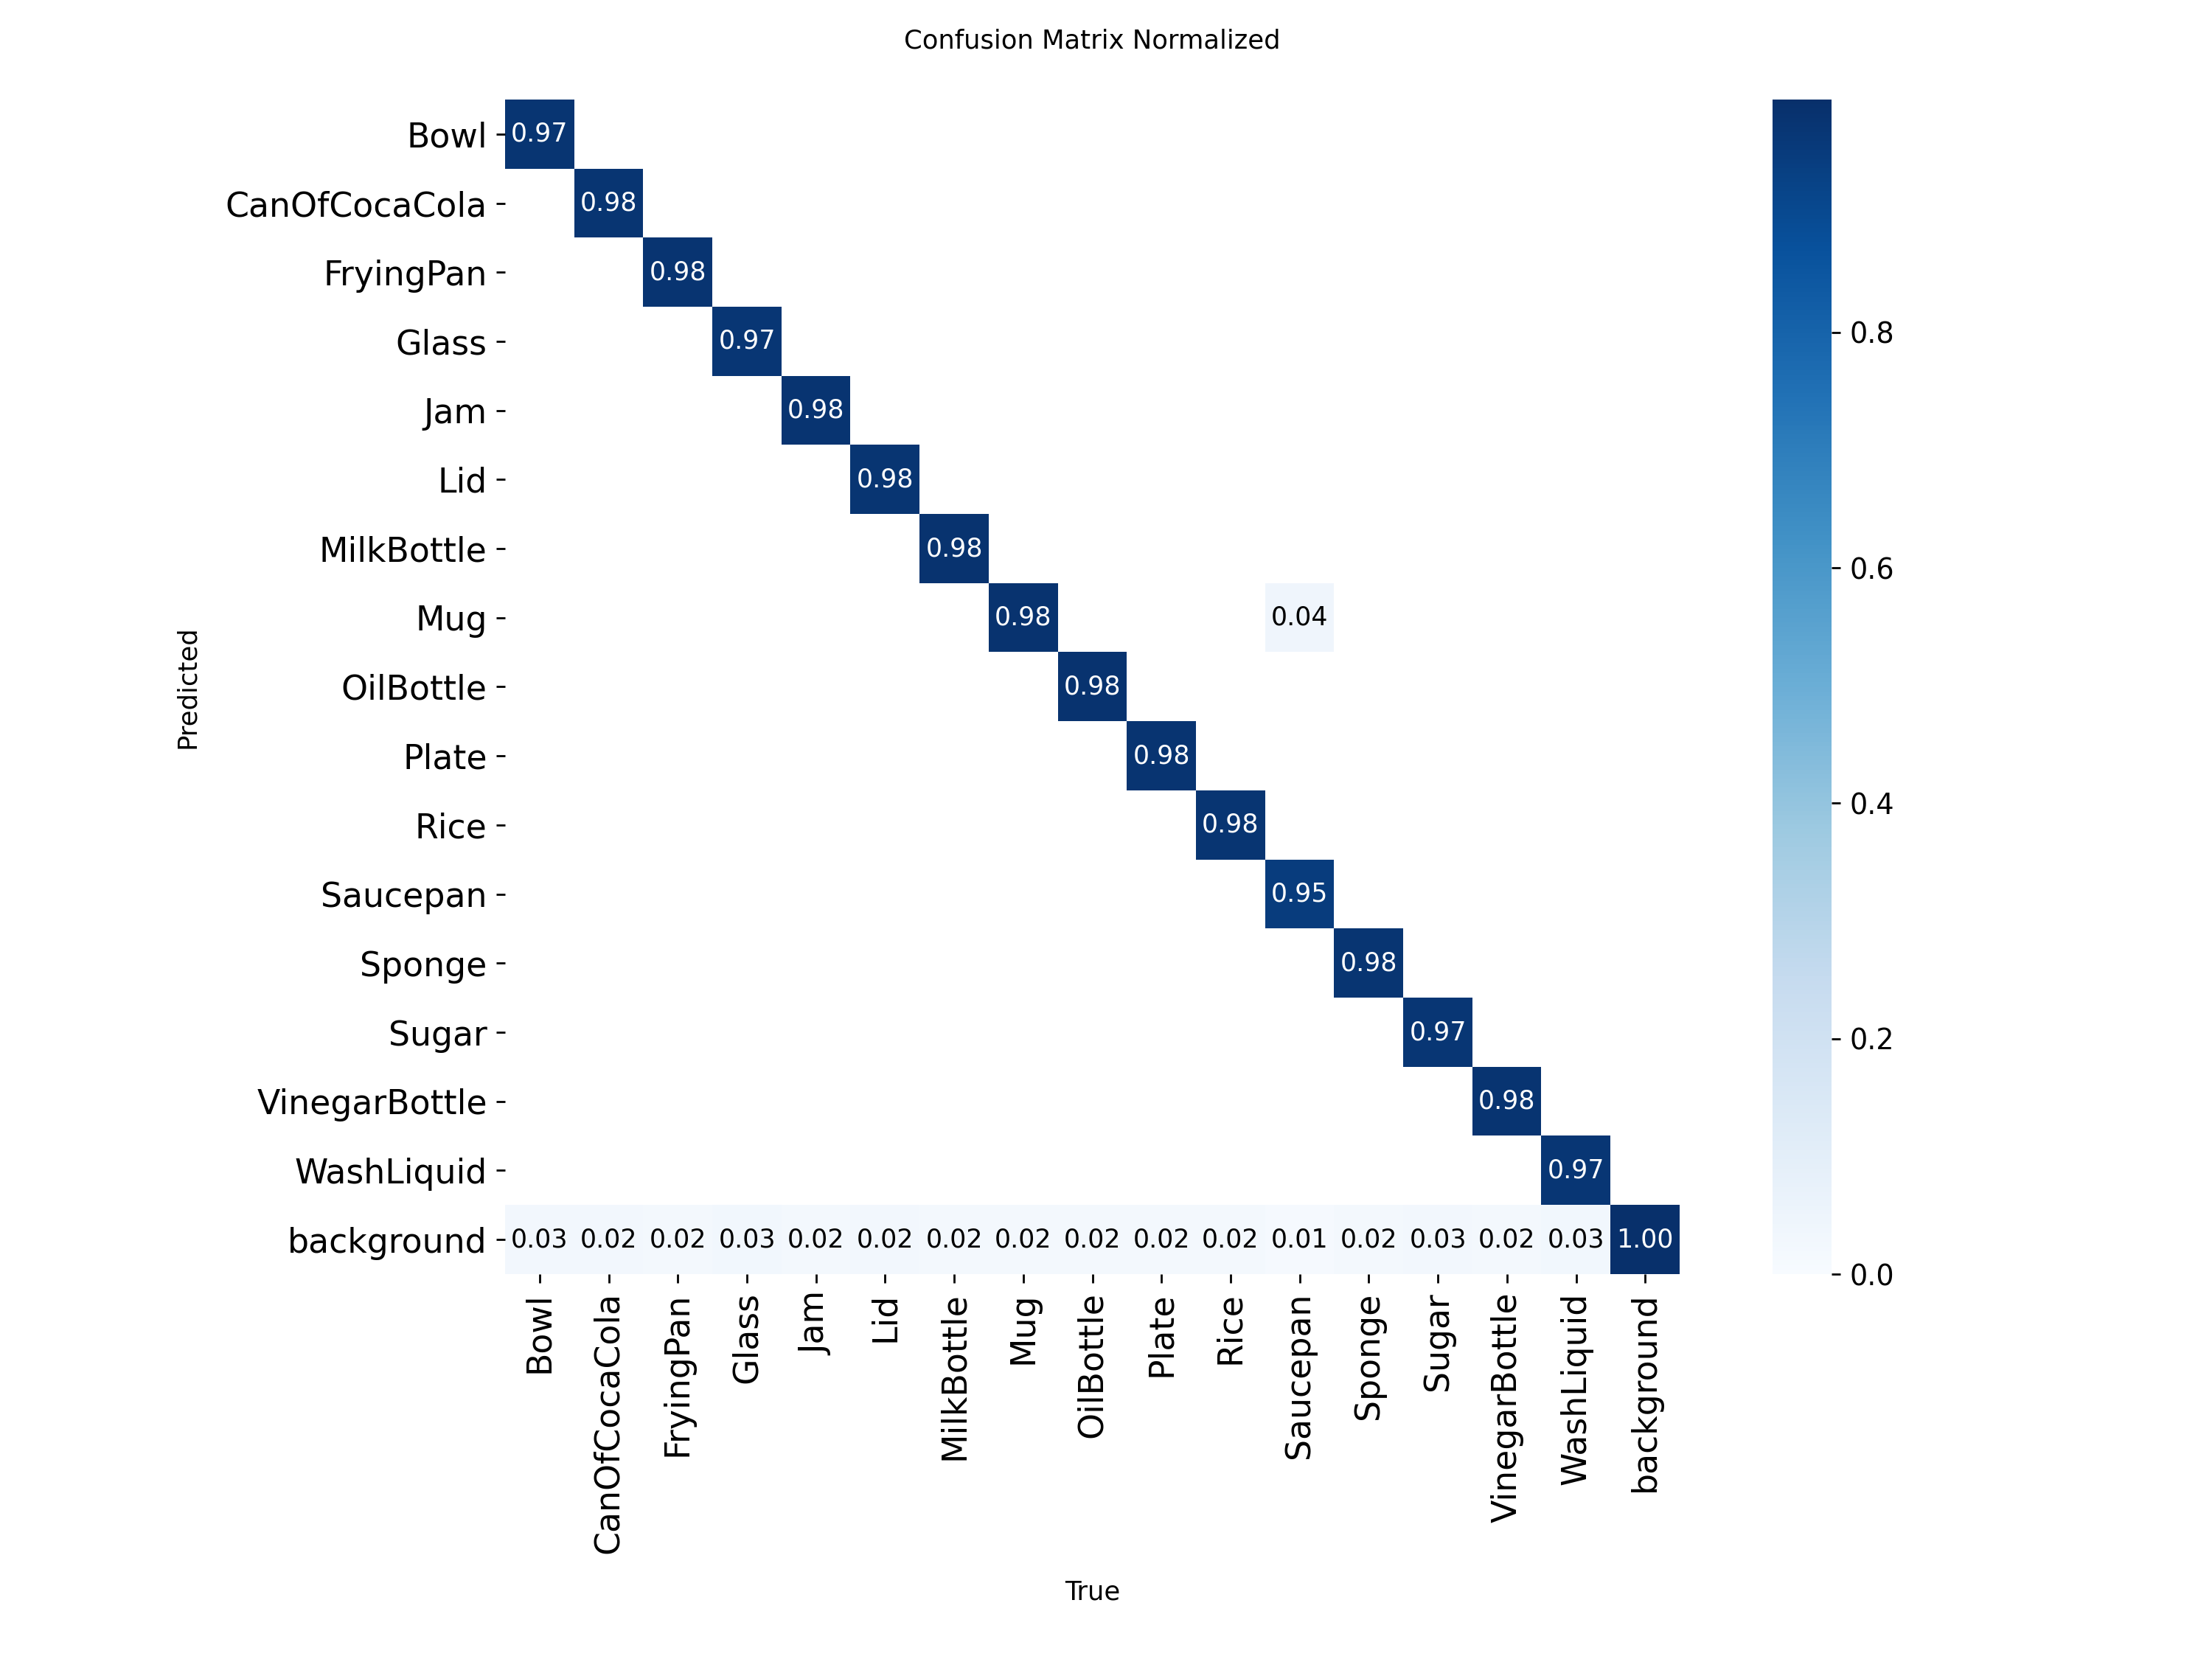
\includegraphics[width=\linewidth]{imgs/sem_conf_norm_mat.png}
    \caption{Normalized Confusion matrix on the validation set}
    \label{fig:finetune-confmat}
\end{figure}

\end{document}